\documentclass{beamer}
%\usetheme{Madrid} % My favorite!
%\usetheme{Boadilla} % Pretty neat, soft color.
%\usetheme{default}
%\usetheme{Warsaw}
%\usetheme{Bergen} % This template has nagivation on the left
\usetheme{Frankfurt} % Similar to the default 
%with an extra region at the top.
%\usecolortheme{seahorse} % Simple and clean template
%\usetheme{Darmstadt} % not so good
% Uncomment the following line if you want %
% page numbers and using Warsaw theme%
 \setbeamertemplate{footline}[page number]
%\setbeamercovered{transparent}
\setbeamercovered{invisible}
% To remove the navigation symbols from 
% the bottom of slides%
\setbeamertemplate{navigation symbols}{ }
%
  \usepackage{graphicx}
  \usepackage{lmodern} %this font kills an annoying compliation warning, and is almost the same as the default.
  \usepackage{subfigure} %for side to side figures
  \usepackage{hyperref} %to create internal links
%\usepackage{bm}         % For typesetting bold math (not \mathbold)
%\logo{\includegraphics[height=0.6cm]{yourlogo.eps}}
%
  \title{Measuring Conspicuous Consumption: a cross-country comparison}
  \author{David Jinkins}
\institute
{
Pennsylvania State University\\
\medskip
{\emph{david.jinkins@gmail.com}}
}
\date{\today}
% \today will show current date. 
% Alternatively, you can specify a date.
%
\begin{document}
%
\begin{frame}
\titlepage
\end{frame}
%
\section{Introduction}

\begin{frame}
  \frametitle{Motivation}
  	\begin{itemize}
           \item Signaling with consumption
	     \begin{itemize}
	       \item Why do people buy expensive watches? 
	       \item This paper: to signal well-being.
	     \end{itemize}
	   \item Well-being (wealth) is unobservable
	     \begin{itemize}
		\item In this paper, your social circle judges your well-being based on your consumption of a single good.
		\item Example: iPad in one social circle, brand-name clothing in another, vacations to exotic locales in another.
	     \end{itemize}
	   \item Why do people care about social beliefs?
	     \begin{itemize}
	       \item Maybe they just do--ex: post-mortem donations.
	       \item Maybe social beliefs are a stepping stone.
	       \item If first, this is a structural model.  If second, this is a reduced form model.
	     \end{itemize}
	\end{itemize}
\end{frame}
%
\begin{frame}
  \frametitle{Preview of Results}
  	\begin{itemize}
           \item Estimation of utility parameters  
	     \begin{itemize}
	       \item The utility function will loosely look like this:
		 \[ 
		   (1-\alpha) u(C) + \alpha E(u|C)
		 \]
	         The first term is fundamental utility, and the second is social belief.
	       \item Americans care about utils of social belief about 1/6 as much as they care about utils of consumption ($\alpha = .1458$).
	       \item Chinese care about utils of social belief about 1/4 as much as they care about utils of consumption ($\alpha = .2$).
	     \end{itemize}
	   \item Taxes on visible goods
	     \begin{itemize}
		\item I propose a tax on visible goods which dramatically increases social welfare.
		\item Median welfare increase is XX\%.
		\item Almost pareto efficient - only XX\% harmed.
	     \end{itemize}
	\end{itemize}
\end{frame}
%
\begin{frame}
  \frametitle{Recent Related literature}
  	\begin{itemize}
           \item Theory of consumption signaling:  
	     \begin{itemize}
	       \item Ireland(1994,JPubEcon),	     
	       \item Heffetz(2007,mimeo)
	     \end{itemize}
	   \item Empirical studies of consumption signaling: 
	     \begin{itemize}
		\item Charles, Hurst, and Roussanov(2009,QJE),
		\item  Heffetz(2012,REStat) 
	     \end{itemize}
	   \item Relative consumption and social status
	     \begin{itemize}
		\item Luttmer(2004,mimeo),
		\item  Arrow and Dasgupta(2009,TheEconJrnl), 
		\item  Clark, Frijters, and Shield(2008,JEL)
	     \end{itemize}
	   \item Chinese Conspicuous Consumption
	     
	\end{itemize}
\end{frame}
%
\section{Model}
\begin{frame}
  \frametitle{Environment}
  \begin{itemize} 
    \item Wealth is exogenous.
    \item There are I goods, and no saving.
    \item The price vector P is exogenous.
    \item Consumers choose a consumption vector C.
    \item Preferences differ across consumers, but are known within the social circle.
    \item Within each social circle, only expenditures on a single good category are observable. 
  \end{itemize}
\end{frame}
% 
\begin{frame}
  \frametitle{Preferences}
   \begin{itemize} 
     \item Social beliefs are described by the I functions $g_i:c_i,\Theta \rightarrow C$
    \item Following Ireland(1994) and Heffetz(2007), utilty has the following form:
      \[
	U(C,\theta,i) = (1-\alpha) u(C,\theta) + \alpha u(g_i(c_i,\theta),\theta)
      \]
    \item $u$ is called the fundamental utility function.
    \item $\theta$ is the preference heterogeneity.
  \end{itemize}
\end{frame}
%
\begin{frame}
  \frametitle{Equilibrium concept}
   \begin{itemize} 
     \item An equilibrium is a set of I belief functions $\{g_i\}$ and a set of $I$ consumption functions $\{C^i\}$ such that:  
       \begin{enumerate}
	 \item For all $i,\theta$, $C^i(\theta)$ solves the consumer's problem given $g_i$. 
	 \item For all $i,\theta$, $g_i(c_i^i(\theta),\theta) = C^i(\theta)$
       \end{enumerate}
     \item This is a standard ``separating equilbrium'' ala Spence.
  \end{itemize}
\end{frame}
%
\begin{frame}
  \frametitle{Solving the Model}
  \begin{itemize}
    \item Substituting optimal unobserved expenditures into the individual's problem, with some manipulation we can write:
  \end{itemize}
      \[
	U(C,\theta) = \theta_v \ln C_v + \left(1-\alpha \right)\hat{\theta} \ln (W-P_v C_v)  + \alpha \hat{\theta} \ln\left((h_v(C_v,\theta)\right) + \psi
      \]
      \hspace{.75cm} $\hat{\theta}$ and $\psi$ are known functions of $\theta$. $h_v$ is belief about $W-P_v C_v$.
      \begin{itemize}
    \item The FOC is then:
      \[
	h_v'(C_v,\theta) = \frac{1}{\alpha}\left(\left( 1-\alpha \right)P_v-\frac{\theta_v}{\hat{\theta}}\frac{h(C_v)}{C_V}  \right)	
      \]
    \item The solution to this differential equation is:
      \[
	h(C_v) = \frac{\hat{\theta}(1-\alpha)}{\theta_v + \alpha \hat{\theta}}P_v C_v + K C_v^{\frac{\theta_v}{\alpha \hat{\theta}}} 
      \]
    \item $K$ is pinned down by lowest possible wealth level.
  \end{itemize}
 \end{frame}
 %
 \section{Data}
 \begin{frame}
	\frametitle{American Data}
	\begin{itemize} 
	  \item Three types of data.
	    \begin{enumerate}
	      \item NBER Consumer Expenditure Extracts.
		\begin{itemize}
		  \item Annual cross-section of consumer expenditures.
		  \item Expenditures broken into categories.
		  \item Demographic information.
		\end{itemize} 
	      \item BLS Relative Price Data
		\begin{itemize}
		  \item Broken down by year and good category.
		  \item Categories intentionally correspond with consumer expenditure data.
		\end{itemize}
	      \item Heffetz Vindex data
		\begin{itemize}
		  \item A telephone survey conducted by Ori Heffetz.
		  \item How ``visible'' are different types of consumption. FLAG survey question
		  \item A single year, broken down by demographics.  
		\end{itemize}
	    \end{enumerate}
	  \item Unit of observation is the household.
	\end{itemize}
 \end{frame}
 %
 \begin{frame}
   \frametitle{Log Expenditure Shares on Log Expenditure by Category}
   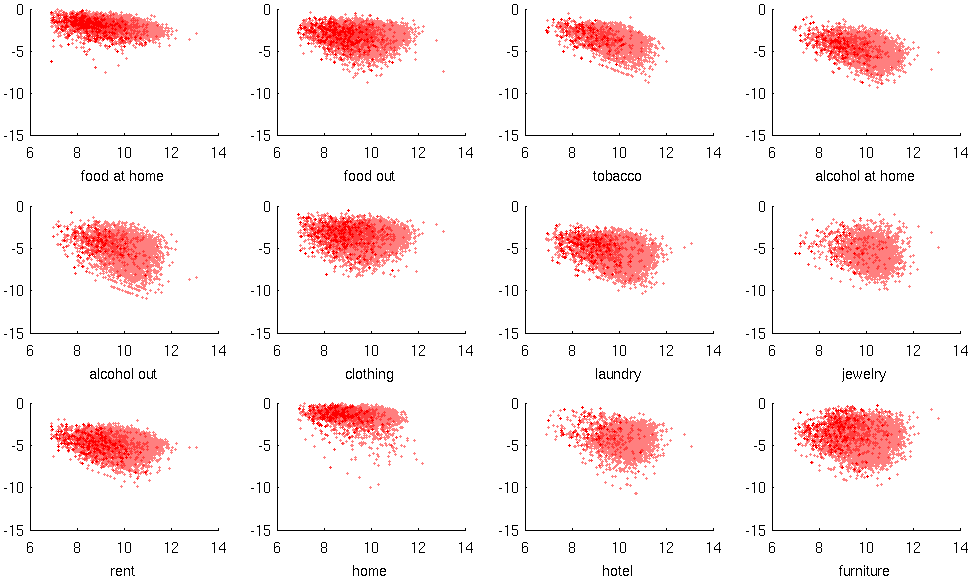
\includegraphics[scale = .70]{pics/shares_cropped_cropped.pdf}
 \end{frame}
 %
 \begin{frame}
   \frametitle{Vindex for blacks under 40}
 \begin{figure}
   \centering
   \mbox{\subfigure{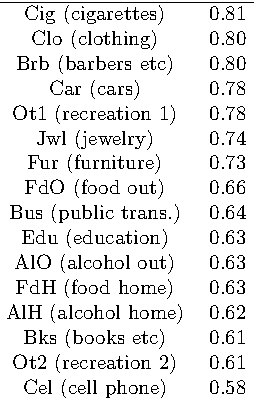
\includegraphics[scale=1]{pics/Vindex_example1.pdf}}\quad
   \subfigure{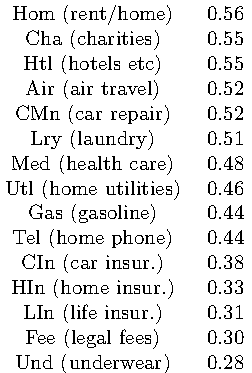
\includegraphics[scale=1]{pics/Vindex_example2.pdf} }}
 \end{figure}
 \end{frame}
 %
 \begin{frame}
   \frametitle{Chinese Data}
   \begin{itemize}
     \item Two types of data:
     \begin{enumerate}
       \item Chinese Household Income Project expenditure data.
         \begin{itemize}
           \item Academic survey, publicly available from University of Michigan.
           \item Urban consumption expenditure survey for 1995 and 2002.
           \item Consumption broken into categories.
         \end{itemize}
       \item Relative Price data from the China Statistical Yearbook.
         \begin{itemize}
          \item Prices broken down into categories with rural/urban distinction.
         \end{itemize}
     \end{enumerate}
   \item We will use the American visibility survey in the Chinese estimation.
 \end{itemize}
 \end{frame}
 %
 \section{Estimation}
 \begin{frame}[label=comeback]
  \frametitle{Assumptions}
  \begin{itemize}
    \item Primary goal is to get $\alpha$, the importance of signaling in utility.
    \item Assume that Cobb-Douglas parameters $\theta$ are distributed independent log-normal with a mass-point at zero.
      \begin{itemize}
	\item The mass-point is necessary because data is quite sparse.         
	\item The log-normal assumption is due to shape of the data. 
      \end{itemize}
\hyperlink{zeros}{\beamergotobutton{data-sparse}} 
\hyperlink{logn}{\beamergotobutton{data-logn}}
    \item Assume that the observed good is drawn in proportion to Heffetz relative visibilities, which differ demographically.
      \begin{itemize}
	\item For technical reasons which simplify estimation, I assume that food at home is never the observed good.
      \end{itemize}
     \item This specification leads 85 free parameters to be estimated.
  \end{itemize}
 \end{frame}
%  
\begin{frame}
  \frametitle{EM Procedure}
  \begin{itemize}
    \item Since the observation type of each household's social circle is an unobservable latent variable, we use an EM estimation proceedure.
    \item Estimation proceeds in two steps:
      \begin{enumerate}
	\item Given a vector of observation types, solve for the most likely utility parameters.
	\item Given utility parameters, solve for the most likely observation types.
      \end{enumerate}
    \item Continue this process until step 2 does not change the list of observation types.
  \end{itemize}
\end{frame}
\begin{frame}
  \frametitle{Identification}
  \begin{itemize}
    \item No formal results on identification.
    \item We have price variation over time in both data sets.
    \item Regardless of demographic, all households draw utility parameters from the same distribution.  
    \item Differences in consumption between demographics are what pins down $\alpha$.
    \item Since we do not have demographic variation in China, identification of $\alpha$ is off of functional form assumptions.
  \end{itemize}
\end{frame}
%
\section{Results}
\begin{frame}
  \frametitle{American Parameter Estimates}
\begin{table}
	\begin{center}
	  \small
		\begin{tabular}{|l|c c |c c |c c|}
			\hline
			Good Cat & $\mu$ & std err      & $\sigma$ & std err       & $pr(\gamma_j =  0)$ & std err\\
			\hline
			FdO & -1.2106 &  (0.0002) &  1.1823 & (0.0005) &   0.0836 & (0.0038)\\ 
			\hline
			Cig & -6.1907 &  (0.0022) & 11.4001 & (0.0512) &   0.8274 & (0.0054)\\ 
			\hline
			AlH & -2.7418 &  (0.0002) &  1.2418 & (0.0006) &   0.4760 & (0.0070)\\ 
			\hline
			AlO & -3.0832 &  (0.0003) &  1.6011 & (0.0010) &   0.5032 & (0.0070)\\ 
			\hline
			Clo & -1.4358 &  (0.0002) &  1.1580 & (0.0005) &   0.0938 & (0.0040)\\ 
			\hline
			Lry & -3.3559 &  (0.0002) &  1.3826 & (0.0007) &   0.3102 & (0.0065)\\ 
			\hline
			Jwl & -5.3608 &  (0.0015) &  8.1810 & (0.0228) &   0.6604 & (0.0067)\\ 
			\hline
			Brb & -2.6958 &  (0.0002) &  1.0096 & (0.0004) &   0.1530 & (0.0050)\\ 
			\hline
			Hom &  0.3824 &  (0.0002) &  0.8689 & (0.0004) &   0.7046 & (0.0065)\\ 
			\hline
			Htl & -2.4135 &  (0.0002) &  1.3596 & (0.0007) &   0.6360 & (0.0068)\\ 
			\hline
			Fur & -1.9858 &  (0.0002) &  1.4964 & (0.0008) &   0.2570 & (0.0061)\\ 
			\hline
			Utl & -0.8731 &  (0.0001) &  0.7561 & (0.0002) &   0.0960 & (0.0041)\\ 
			\hline
			Tel & -1.6308 &  (0.0001) &  0.9058 & (0.0003) &   0.0360 & (0.0025)\\ 
			\hline
			HIn & -1.5132 &  (0.0002) &  1.1389 & (0.0005) &   0.4102 & (0.0069)\\ 
			\hline
		        \hline	
			$\alpha$ & 0.1459 & (0.0071) & & & & \\
			\hline
		\end{tabular}
	\end{center}
	\label{tab:parest}
\end{table}
\end{frame}
 %
 \begin{frame}
   \frametitle{Simulated vs Actual Expenditure Shares by Category}
 \begin{figure}
   \centering
   \mbox{\subfigure{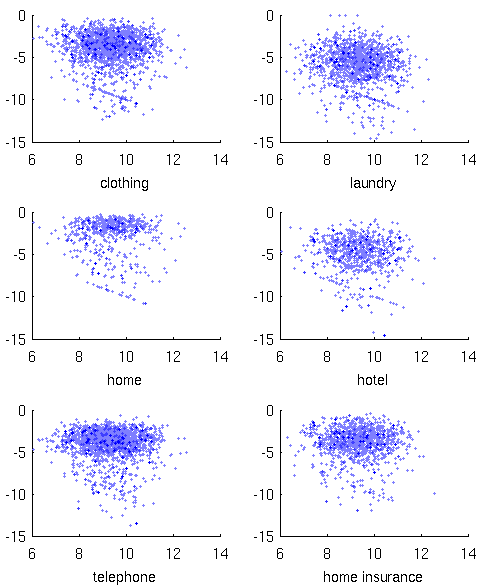
\includegraphics[scale=.7]{pics/shares_fake_cropped_cropped.pdf}}\quad
   \subfigure{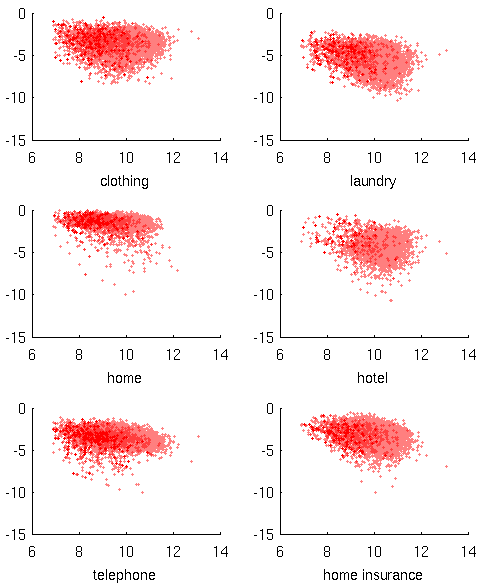
\includegraphics[scale=.7]{pics/shares_cropped_compare.pdf} }}
 \end{figure}
  \end{frame}
 %
  \begin{frame}
    \frametitle{Vindex vs Estimated Observation Type Proportions}
    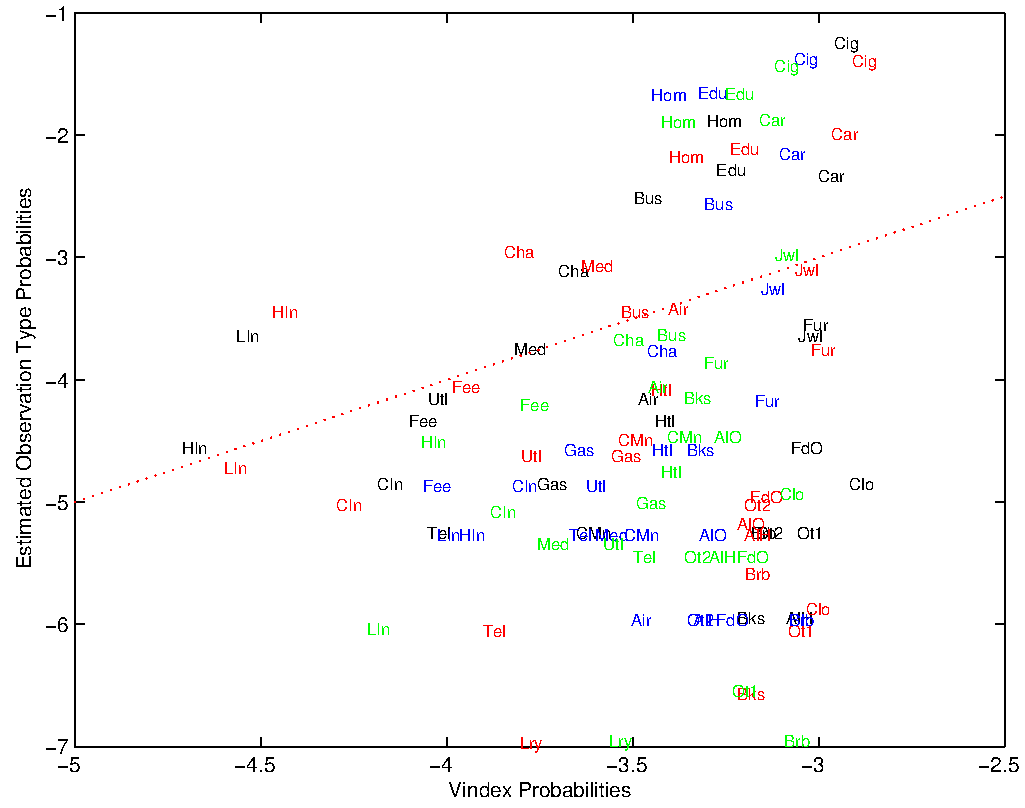
\includegraphics[scale=.58]{pics/vinmatch_cropped.pdf}
  \end{frame}
 %
  \begin{frame}
    \frametitle{Welfare Loss Due to Signaling Motive by Obs. Type} 
    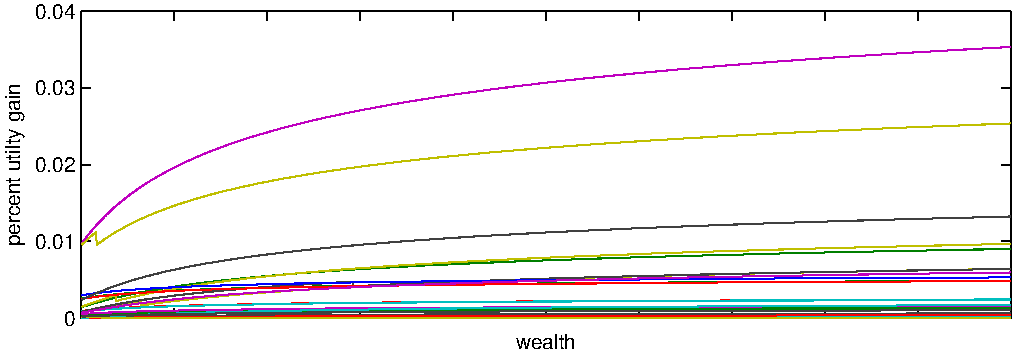
\includegraphics[width=11cm, height=8cm]{pics/uchnge_cropped_nohouse.pdf} 
  \end{frame}
  %
  \begin{frame}
    \frametitle{Chinese Parameter Estimates}
    TO BE ADDED
  \end{frame}
  %
  \begin{frame}
    \frametitle{Discussion of Chinese vs American estimates}
    TO BE ADDED
  \end{frame}
  %
  \section{Tax}
  \begin{frame}
    \frametitle{Tax Scheme}
    \begin{itemize}
      \item The basic idea is an excise tax on each good.
      \item Gov't revenue is passed back to households in proportion to wealth.
      \item Intuitively, households overconsume visible goods.  The tax raises the price of visible goods, but wealth unaffected $\rightarrow$ less distortion.
      \item In the exercise that follows, prices and wages are fixed (think perfect competition).
      \item In the paper, I show that this tax scheme will not affect household budget share decisions. 
      \item To find optimal taxes, I define the social welfare function to be the sum of all individual utilities.
    \end{itemize}
  \end{frame}
  \begin{frame}
    \frametitle{Optimal Taxes} 
\begin{table}
	\begin{center}
		\begin{tabular}{|l|c|l|c|}
			\hline
			\textbf{Good Cat} & \textbf{Tax} & \textbf{Good Cat} & \textbf{Tax}\\
			\hline
			FdH &  3.7860 & HIn &  0.3863\\
			\hline         
			FdO &  1.5188 & Med &  0.7386\\ 
			\hline        
			Cig &  8.4272 & Fee &  0.0000\\ 
			\hline       
			AlH &  2.1151 & LIn &  0.5304\\ 
			\hline      
			AlO &  0.0761 & Car &  1.1046\\ 
			\hline     
			Clo &  1.1873 & CMn &  2.0361\\ 
			\hline    
			Lry &  0.0000 & Gas &  2.2456\\ 
			\hline   
			Jwl &  3.1023 & CIn &  0.5941\\ 
			\hline  
			Brb &  0.0000 & Bus &  2.7202\\ 
			\hline 
			Hom &  8.8748 & Air &  2.2799\\ 
			\hline
			Htl &  0.0733 & Bks &  0.0000\\ 
			\hline
			Fur &  0.9623 & Ot1 &  0.0000\\ 
			\hline
			Utl &  1.9966 & Ot2 &  1.5486\\ 
			\hline
			Tel &  0.9322 & Edu &  1.2739\\ 
			\hline
			HIn &  0.3863 & Cha &  1.3754\\ 
		        \hline
		\end{tabular}
	\end{center}
	\label{tab:opttax}
\end{table}
  \end{frame}
  %
  \begin{frame}
    \frametitle{Correlation of Optimal Taxes with Obs Type Proportion}
    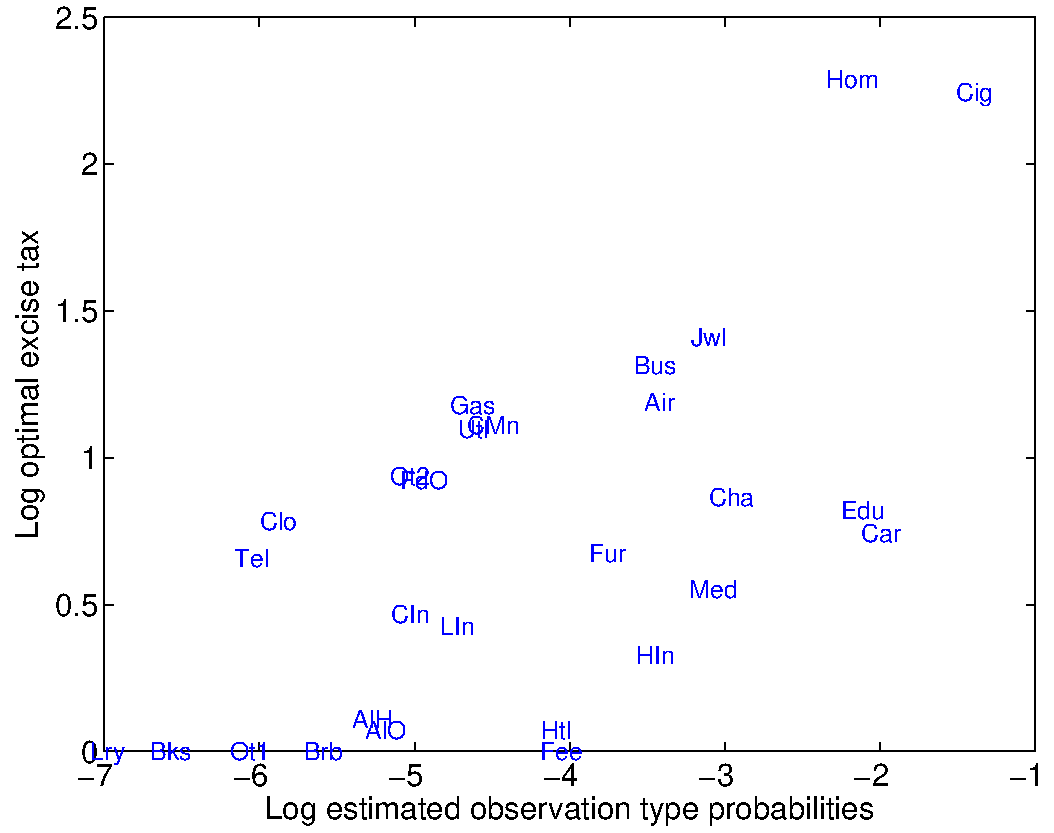
\includegraphics[scale=.55]{pics/tvscat_cropped.pdf} 
  \end{frame}
  %
  \begin{frame}
    \frametitle{Utility Change after Tax Implementation}
    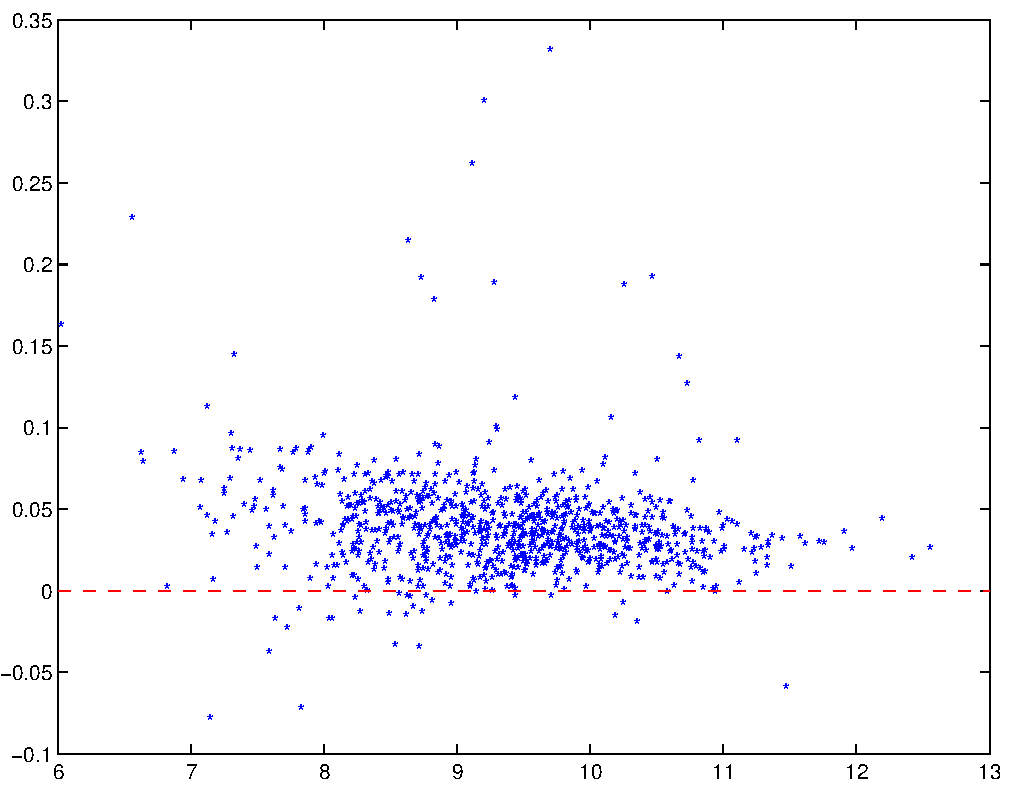
\includegraphics[scale=.55]{pics/taxscat_cropped.pdf} 
  \end{frame}
  %  
  \begin{frame}
    \frametitle{Taxes: Bottom Line}
    \begin{itemize}
      \item There are significant welfare gains from the proposed tax scheme.
      \item Tax scheme is largely in line with what is implemented in the real world.
      \item Largest optimal taxes are on property, cigarettes, and jewelry.
    \end{itemize}
    \end{frame}
    %
    \begin{frame} 
      \frametitle{Conclusion}
      TO BE ADDED
    \end{frame}
    %
    \begin{frame}[label=zeros]
      \frametitle{Expenditures Data is Sparse}
	  \footnotesize
\begin{tabular}{|l|c|l|c|}
	\hline
\textbf{Category} & \textbf{Zero Expenditure} & \textbf{Category} & \textbf{Zero Expenditure}\\
	\hline
Clo (clothing)       & 0.11 & Edu (education)      & 0.70\\ 
	\hline              
Cig (cigarettes)     & 0.60 & Hom (rent/home)      & 0.57\\ 
	\hline             
Car (cars)           & 0.47 & FdH (food home)      & 0.02\\ 
	\hline              
Fur (furniture)      & 0.26 & Htl (hotels etc)     & 0.62\\ 
	\hline              
Ot1 (recreation 1)   & 0.16 & Air (air travel)     & 0.67\\ 
	\hline              
Jwl (jewelry)        & 0.64 & Bus (public trans.)  & 0.73\\ 
	\hline              
FdO (food out)       & 0.10 & CMn (car repair)     & 0.24\\ 
	\hline              
AlH (alcohol home)   & 0.49 & Cha (charities)      & 0.58\\ 
	\hline             
AlO (alcohol out)    & 0.51 & Gas (gasoline)       & 0.11\\ 
	\hline              
Ot2 (recreation 2)   & 0.10 & Lry (laundry)        & 0.33\\ 
	\hline              
Brb (barbers etc)    & 0.17 & Med (health care)    & 0.25\\ 
	\hline             
Bks (books etc)      & 0.48 & Tel (home phone)     & 0.06\\ 
	\hline              
Edu (education)      & 0.70 & Utl (home utilities) & 0.12\\ 
	\hline              
Hom (rent/home)      & 0.57 & Fee (legal fees)     & 0.36\\ 
	\hline              
FdH (food home)      & 0.02 & CIn (car insur.)     & 0.35\\ 
	\hline              
Htl (hotels etc)     & 0.62 & LIn (life insur.)   & 0.54 \\ 
	\hline              
Air (air travel)     & 0.67 & HIn (home insur.)   & 0.41 \\ 
	\hline
\end{tabular}

  \hyperlink{comeback}{\beamergotobutton{go back}}
\end{frame}
%
\begin{frame}[label=logn]
  \frametitle{Histogram of Log Expenditure Shares by Category}
  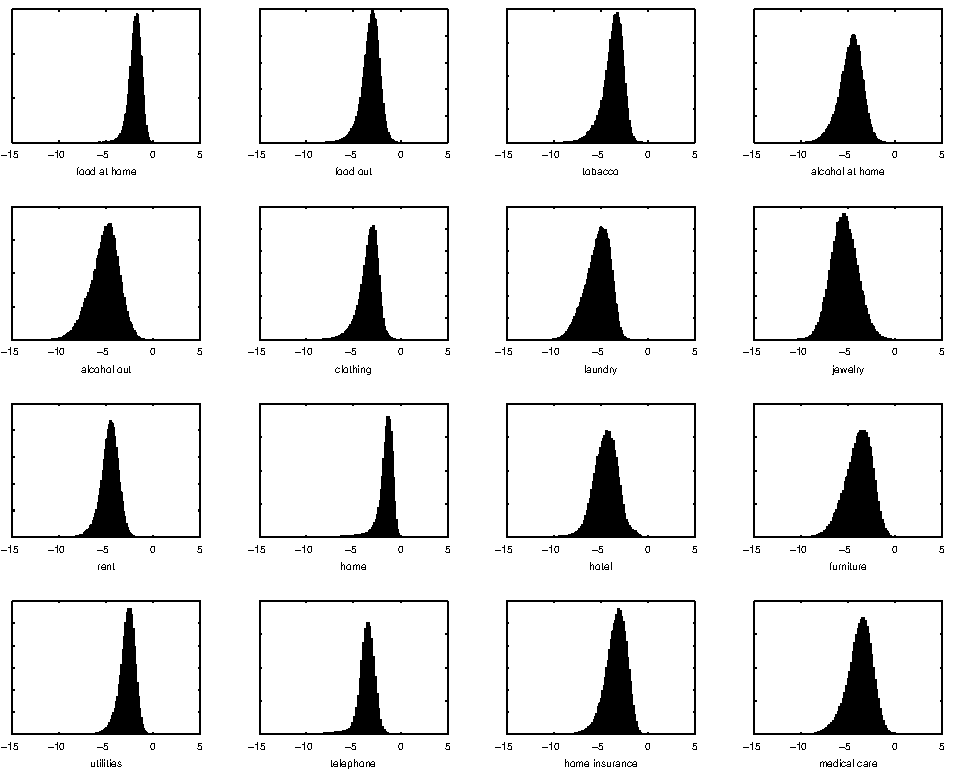
\includegraphics[width=11cm, height=7.5cm]{pics/shrplot_cropped.pdf}

  \hyperlink{comeback}{\beamergotobutton{go back}}
\end{frame}
\end{document}
